\documentclass[conference]{IEEEtran}
\IEEEoverridecommandlockouts

\usepackage{amssymb}
\usepackage[table]{xcolor}
\usepackage{xspace}
\usepackage{booktabs}
\usepackage{amsmath}
\usepackage{graphicx}
\usepackage{algorithm}
\usepackage{algpseudocode}
\usepackage{float}
\usepackage{cite}
\usepackage{subcaption}
\usepackage{makecell}
\usepackage{xurl}
\usepackage{tikz}
\usetikzlibrary{arrows.meta, positioning, fit, calc}

% ---- Macros ----
\newcommand{\smarm}{SMARM\xspace}
\newcommand{\tdis}{$t_{\mathrm{disabled}}$\xspace}
\newcommand{\FAR}{FAR\xspace}
\newcommand{\smarmcopy}{SMARM+Copy\xspace}
\newcommand{\smarmlock}{SMARM+Lock\xspace}

\newcommand\oak[1]{\textcolor{red}{OAK: #1}}
\newcommand\ben[1]{\textcolor{blue}{#1}}

\begin{document}

\title{Towards Fully Interruptible Shuffled Measurement for Remote Attestation}

% DOUBLE-BLIND: comment out \author before submitting if required
\author{
  \IEEEauthorblockN{Amarin Laohajirapan, Norrathep Rattanavipanon}
  \IEEEauthorblockA{College of Computing,
    Prince of Songkla University, Phuket Campus, Thailand \\
    norrathep.r@psu.ac.th}
}

\maketitle

% ================================================================
\begin{abstract}
Remote attestation (RA) detects software compromise on IoT devices, but
classical RA keeps interrupts disabled for a full memory scan and can
block real-time work for hundreds of milliseconds.
SMARM instead measures memory in a secret shuffled order so attestation
can be interrupted between blocks while still resisting
\emph{roving malware}.
The original design was evaluated on a formally verified microkernel
stack, not on widely used production RTOSes.
We port SMARM to FreeRTOS on ARM TrustZone-M and show that, although
interrupts are re-enabled between blocks, hashing each block with
interrupts disabled still breaks common real-time periods when the block
size grows on commodity Cortex-M33 hardware.
We study two TrustZone-M enhancements that keep the block snapshot
atomic while allowing hash work to coexist with interrupts.
\emph{\smarmcopy} disables interrupts only around a short memory copy
into Secure RAM, then hashes with interrupts enabled.
\smarmlock{} instead uses brief \emph{memory locking} so the target
block stays protected during an in-place hash, with no copy buffer
(instantiated on TrustZone-M via SAU reprogramming).
Both restore Frequency Accuracy Ratio
(FAR)~$\approx 1.0$ for all tested block sizes up to $B{=}4096$~bytes
and workloads from $10$ to $1000$~Hz on STM32L552ZE with FreeRTOS.
\end{abstract}

\begin{IEEEkeywords}
Remote attestation, IoT security, memory locking, TrustZone-M, RTOS,
SMARM, interrupt latency
\end{IEEEkeywords}

% ================================================================
\section{Introduction}
\label{sec:intro}

Modern societies increasingly depend on Internet-of-Things (IoT) devices across domains ranging from smart factories, where industrial sensors support monitoring and automation, to smart homes, where devices such as smart lights and robotic vacuum cleaners improve convenience. 
Since many IoT devices are designed to be inexpensive and energy-efficient, they typically operate on resource-constrained microcontrollers (MCUs) with limited RAM, flash storage, and energy budgets. These constraints often preclude sophisticated monolithic operating systems and the malware defenses available on higher-end devices.

Remote attestation (RA)~\cite{eldefrawy2012smart,nunes2019vrased,eldefrawy2017hydra} has emerged as an inexpensive technique for detecting malware compromise on resource-constrained IoT devices. In RA, an IoT device, called the \emph{prover}, executes a measurement routines that hashes its software image (i.e., the code stored in flash memory) and returns the measurement result in an authenticated response (e.g., using a message authentication code (MAC) or digital signature). 
An external trusted party, called the \emph{verifier}, compares this measurement against that of the expected software image to determine whether the prover's software has been modified and hence be able to deduce whether a malware compromise happens on the prover.

Traditional RA requires the measurement routine to execute atomically with interrupts disabled. This atomic execution is necessary to prevent \emph{roving malware} from evading detection by relocating itself to a region that has already been measured. On low-end MCUs, however, the resulting non-preemptible interval can exceed $450$~ms~\cite{nunes2019vrased}. Such prolonged interrupt disablement can severely interfere with real-time applications whose correctness depends on completing time-critical tasks within their deadlines.

To relax the atomicity requirement, SMARM~\cite{carpent2018smarm} introduces a new technique, called \emph{shuffled measurement}, which permits interrupts between the measurements of individual memory blocks. To defend against roving malware, SMARM measures the blocks comprising the software image in a random and secret order. Because malware does not know which blocks have already been measured, it cannot reliably relocate itself to an inspected block to evade detection. Although this approach does not provide the deterministic protection of fully atomic measurement, it makes evasion probabilistically difficult while reducing the non-preemptible interval from the measurement of the entire software image to that of a single block.

Despite this improvement, SMARM's maximum non-preemptible interval remains determined by its block size. Prior work~\cite{smarmplus2026,carpent2018smarm} shows that using larger blocks can reduce the total attestation time by lowering per-block processing overhead. However, a larger block also takes longer to measure, thereby extending each non-preemptible interval and potentially delaying time-critical tasks beyond their deadlines. Conversely, smaller blocks shorten these intervals but increase the number of blocks and the associated computational overhead, resulting in longer attestation times and greater energy consumption. SMARM therefore exposes an inherent tradeoff between real-time responsiveness and energy efficiency, which is particularly problematic for battery-powered IoT devices.

Motivated by this observation, we propose two independent enhancements to shuffled measurement that further shorten its non-interruptible periods, allowing the technique to coexist with a broader range of time-sensitive applications. 
Our contributions are as follows:

\begin{itemize}
\item We propose \smarmcopy, which reduces each non-interruptible period from the time required to hash one memory block to the substantially shorter time required to copy that block.

\item Since \smarmcopy's non-interruptible period remains proportional to the block size, we further propose \smarmlock, which uses \emph{memory locking} so the block snapshot stays atomic while HMAC runs with interrupts enabled. Each block still needs brief interrupt-disable windows for lock and unlock (with \texttt{DSB}/\texttt{ISB} around SAU updates); on our prototype these windows total $87$--$143$ CPU cycles depending on~$B$, far shorter than hashing the block.

\item We implement \smarmcopy and \smarmlock on an STM32 Nucleo-144 board (STM32L552ZE, Cortex-M33 with TrustZone-M)~\cite{stm32nucleo144,stm32l552} running FreeRTOS and evaluate them on real hardware. Our results demonstrate that both mechanisms substantially reduce SMARM's non-interruptible periods, thereby improving their compatibility with time-sensitive embedded applications.

\end{itemize}

% ================================================================
\section{Background}
\label{sec:background}

\subsection{RA Atomicity and SMARM}
At a high level, remote attestation (RA) is a challenge--response
protocol between a resource-constrained \emph{prover} (the IoT device)
and a trusted \emph{verifier}.
The verifier sends a fresh challenge (e.g., a random nonce); the prover
computes an authenticated integrity measurement---typically a message
authentication code (MAC) or digital signature---over its software image
together with that challenge and returns it as attestation evidence; the
verifier checks the evidence against a reference value for the expected
software state.
Classical RA often disables interrupts for the whole measurement so that
\emph{roving malware} cannot move itself while memory is being
hashed~\cite{eldefrawy2012smart,nunes2019vrased}.
SMARM~\cite{carpent2018smarm} instead derives a one-time permutation
$\sigma$ from the verifier challenge and a secret key $k$, then measures
blocks $M_{\sigma(i)}$ one by one, re-enabling interrupts between
blocks. The security claim is not ``malware cannot interrupt''; it is
that malware without knowledge of the remaining secret order cannot
reliably relocate to escape detection, and repeated independent sessions
drive the escape probability down~\cite{carpent2018smarm}.
SMARM requires three security properties:
\begin{enumerate}
  \item \textbf{(S1) Controlled Execution.}
    The attestation service is reachable only through defined
    entry/exit points (on our platform, NSC gates into Secure
    world). Interrupts may be re-enabled only
    \emph{between} block measurements---never in the middle of a
    protected capture step---so malware cannot splice itself into a
    half-measured block.
  \item \textbf{(S2) Key Secrecy.}
    The attestation key $k$ is stored in memory inaccessible to
    untrusted Non-Secure software, so malware cannot forge a valid
    report.
  \item \textbf{(S3) Private Measurement Order.}
    The permutation $\sigma$ is stored in memory inaccessible to
    KFV (known-future-visit) malware, so the adversary cannot
    predict which remaining blocks will be measured next and relocate
    ahead of the scan.
\end{enumerate}
The original SMARM evaluation used a HYDRA/seL4 trust
anchor~\cite{eldefrawy2017hydra,carpent2018smarm}.
A companion report by the same authors~\cite{smarmplus2026} ports the
shuffled protocol to FreeRTOS on TrustZone-M: interrupts are re-enabled
between blocks, but each block is still hashed with interrupts disabled.
We adopt that implementation as our \emph{experimental baseline} when
evaluating Atomic Copy and \smarmlock{}; this paper studies per-block
capture mechanisms rather than extending that port.

\subsection{TrustZone-M Background}

ARM TrustZone-M for Cortex-M~\cite{trustzone2025,an5347} partitions
software on a single MCU into two isolated \emph{worlds}: the
\emph{Secure} world hosts trusted code and secrets, while the
\emph{Non-Secure} world runs the RTOS, applications, and attested
program memory.
The Security Attribution Unit (SAU) and the Implementation Defined
Attribution Unit (IDAU) label each memory region as Secure, Non-Secure,
or Non-Secure Callable (NSC) at the hardware level; Non-Secure software
cannot read or modify Secure regions, and Secure services are reachable
from Non-Secure code only through NSC entry points guarded by the
processor's secure-state transition mechanism.
Our evaluation instantiates SMARM with FreeRTOS in the Non-Secure world
and the attestation service, key~$k$, and permutation~$\sigma$ in Secure
RAM, invoked via NSC (Fig.~\ref{fig:system_model}).
Between consecutive block measurements the RTOS may preempt the
Non-Secure wrapper and run other tasks, including high-priority
real-time workloads (Fig.~\ref{fig:workflow}).

\begin{figure}[!t]
  \centering
  \includegraphics[width=0.92\linewidth]{system-threat-model.pdf}
  \caption{SMARM on FreeRTOS with TrustZone-M. The Non-Secure wrapper
    calls a Secure service through NSC. Key $k$ and permutation
    $\sigma$ stay in Secure RAM.}
  \label{fig:system_model}
\end{figure}

\begin{figure}[!t]
  \centering
  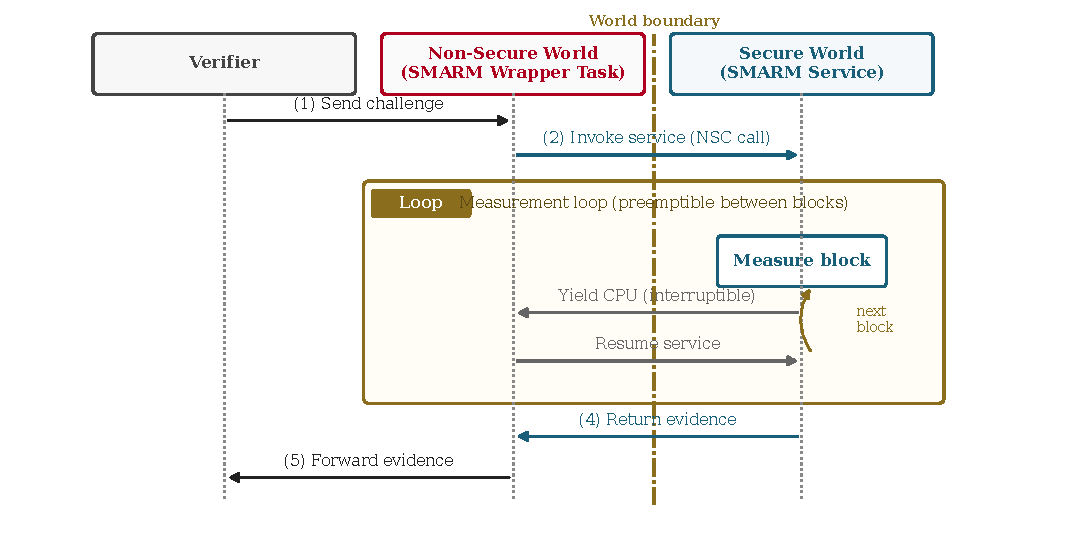
\includegraphics[width=0.92\linewidth]{smarm_workflow.pdf}
  \caption{End-to-end SMARM workflow. Real-time tasks may run between
    consecutive block measurements.}
  \label{fig:workflow}
\end{figure}

Table~\ref{tab:ra_comparison} places traditional RA, SMARM, and our two
enhancements side by side.

\begin{table}[!t]
  \centering
  \caption{Comparison of attestation approaches for real-time IoT devices.}
  \label{tab:ra_comparison}
  \renewcommand{\arraystretch}{1.1}
  \small
  \setlength{\tabcolsep}{2.5pt}
  \begin{tabular}{lcccc}
    \toprule
    \textbf{Approach} &
    \textbf{RT-safe} &
    \makecell{\textbf{Extra} \\ \textbf{RAM}} &
    \makecell{\textbf{Atomic} \\ \textbf{window}} &
    \textbf{RTOS} \\
    \midrule
    Traditional RA~\cite{eldefrawy2012smart} &
      \texttimes & 0 & Full scan & \texttimes \\
    SMARM~\cite{carpent2018smarm} &
      Partial & 0 & Per-block hash & \texttimes \\
    \textbf{Atomic Copy} &
      \checkmark & $+B$ & Per-block copy & \checkmark \\
    \textbf{\smarmlock} &
      \checkmark & 0 & Brief lock; hash IRQ on & \checkmark \\
    \bottomrule
  \end{tabular}
\end{table}

% ================================================================
\section{Motivation}
\label{sec:motivation}

In baseline SMARM, each block update disables interrupts for the full
SHA-256 work on that block. With about $1.1$~MB/s hash throughput on our
board, \tdis grows from $0.062$~ms at $B{=}64$~bytes to $3.75$~ms at
$B{=}4096$~bytes. A $1000$~Hz task has a $1$~ms period, so large blocks
hold the CPU through several missed activations.

Figure~\ref{fig:timing_diagram} sketches the interrupt-disabled windows
for traditional RA, SMARM baseline, and Atomic Copy. Figure~\ref{fig:setup_and_baseline_far}
shows the measured impact: under a $1000$~Hz workload,
$\mathrm{FAR}$ stays near $1.0$ only for $B\leq 1024$~bytes and falls
sharply at $B\geq 2048$~bytes (down to about $0.27$ at $B{=}4096$).

\begin{figure}[!t]
  \centering
  \includegraphics[width=\linewidth]{timing_diagram.png}
  \caption{Interrupt-disabled windows. Traditional RA covers the full
    scan. SMARM limits disability to one block hash. Atomic Copy further
    limits it to one block copy.}
  \label{fig:timing_diagram}
\end{figure}

\begin{figure}[!t]
  \centering
  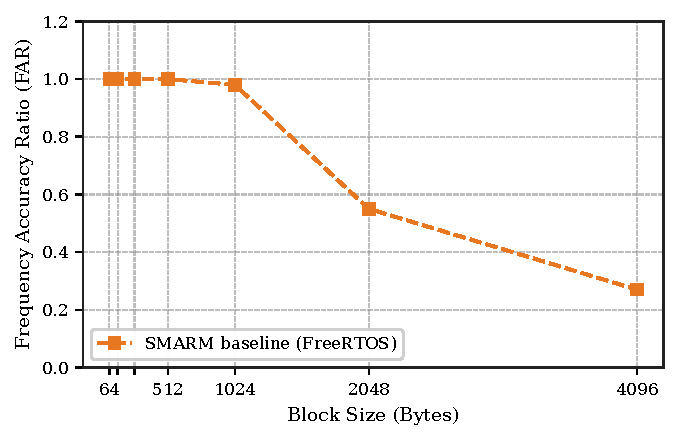
\includegraphics[width=\linewidth]{far_1000.pdf}
  \caption{FAR of baseline SMARM under a $1000$~Hz real-time workload
    across block sizes (FreeRTOS). Values stay near $1.0$ for
    $B\leq 1024$~bytes and drop for larger $B$.}
  \label{fig:setup_and_baseline_far}
\end{figure}

\textbf{Root cause.} Cryptographic hashing itself does not need to be
atomic. What must be atomic is the capture of the block bytes that feed
the hash. The next section presents two ways to protect that capture
while keeping hash work interruptible.

% ================================================================
\section{Design}
\label{sec:design}

\subsection{Atomic Copy}
\label{sec:atomic}

Atomic Copy splits each block step into (i)~an interrupt-disabled
\texttt{Memcpy} into a Secure buffer of size $B$, and (ii)~an
interrupt-enabled \texttt{HMAC.Update} over that buffer
(Fig.~\ref{fig:atomic_copy_workflow}, Algorithm~\ref{alg:atomic_copy}).
Memory copy on our Cortex-M33 is about $17$~MB/s, so
$t_{\mathrm{disabled}}^{\mathrm{copy}}\approx B/17\,\mathrm{MB/s}$,
roughly $15\times$ shorter than hashing under interrupt disable.

\begin{figure}[!t]
  \centering
  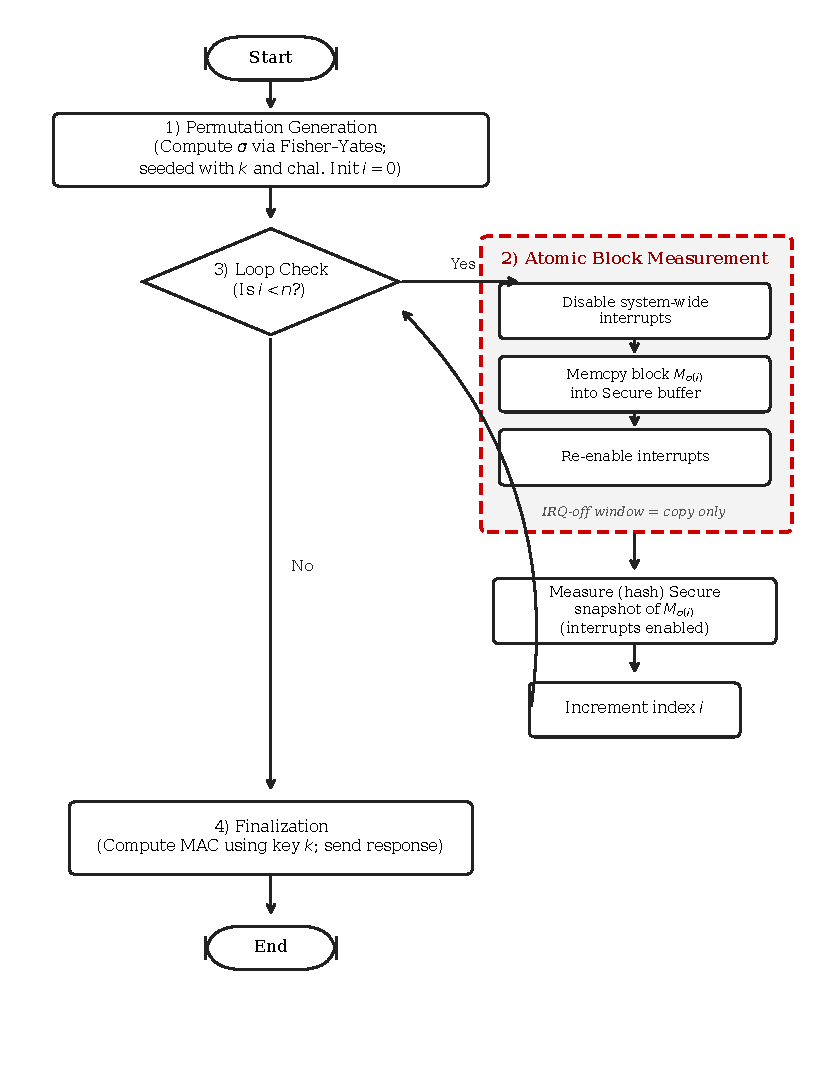
\includegraphics[width=0.92\linewidth]{atomic_workflow.pdf}
  \caption{Atomic Copy flowchart. The dashed region is the short
    interrupt-disabled window (copy only); hashing runs afterward with
    interrupts enabled.}
  \label{fig:atomic_copy_workflow}
\end{figure}

\begin{algorithm}[!ht]
\caption{Atomic Copy Secure Service}
\label{alg:atomic_copy}
\begin{algorithmic}[1]
\Require $n$ blocks, shuffled indices $\sigma$, memory $M$, key $k$
\State \Call{HMAC.Init}{$k$}
\For{$i \gets 0$ to $n-1$}
  \State $\mathit{blk} \gets M[\sigma(i)\cdot B]$
  \State \Call{DisableInterrupts}{}
  \State \Call{Memcpy}{\textit{buf}, \textit{blk}, $B$} \Comment{atomic snapshot}
  \State \Call{EnableInterrupts}{}
  \State \Call{HMAC.Update}{\textit{buf}, $B$} \Comment{interrupts on}
\EndFor
\State \textbf{return} \Call{HMAC.Finalize}{}
\end{algorithmic}
\end{algorithm}

\textbf{Security sketch.} The IRQ-off window covers only the copy, so
the snapshot that feeds HMAC is not half-updated~(S1). Key $k$ and
permutation $\sigma$ remain in Secure RAM~(S2)--(S3); hashing after the
copy uses only Secure buffer contents. We summarize preservation of
(S1)--(S3) for both designs in Section~\ref{sec:security_summary}.

\subsection{Memory Locking (\smarmlock)}
\label{sec:sau}

Atomic Copy costs an extra Secure buffer of size $B$.
\smarmlock{} avoids that buffer through \emph{memory locking}: briefly
reprogramming hardware memory protection so the selected attestation block
is inaccessible to untrusted software while it is hashed in place, then
restoring the prior map before the next block.
On our TrustZone-M prototype, the SAU assigns security attributes to
address ranges~\cite{armv8m-arm,an5347}.
An enabled SAU region is either Non-Secure or Secure/Non-Secure Callable;
addresses not covered by any enabled region are Secure by default.
Attestation uses a dedicated Non-Secure \emph{data window} $|M|$
(separate from Non-Secure application code).
For each shuffled block, two dynamic SAU regions (we use regions~6 and~7)
cover the NS fragments to the left and right of $M_{\sigma(i)}$, leaving
that $B$-byte block outside enabled NS coverage.
The block is then hashed in place with interrupts enabled.
Finally, the window returns to full Non-Secure coverage before the next
block (Fig.~\ref{fig:sau_memory_map}, Fig.~\ref{fig:sau_workflow},
Algorithm~\ref{alg:sau}).
Fig.~\ref{fig:sau_workflow} mirrors the Atomic Copy flowchart, but the
short interrupt-disabled window applies to the SAU lock/unlock sequence
rather than a \texttt{Memcpy}; HMAC still runs with interrupts enabled.

\begin{figure}[!t]
  \centering
  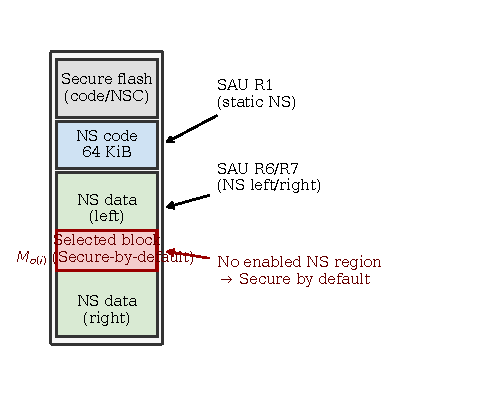
\includegraphics[width=\linewidth]{sau_memory_map.pdf}
  \caption{Memory locking over dedicated Non-Secure data window $|M|$
    (TrustZone-M SAU).
    Region~1 statically marks Non-Secure application code.
    Regions~6/7 dynamically cover the NS byte ranges on either side of the
    selected block $M_{\sigma(i)}$; with no enabled NS region over that
    $B$-byte block, it is Secure-by-default during measurement.}
  \label{fig:sau_memory_map}
\end{figure}

\begin{figure}[!t]
  \centering
  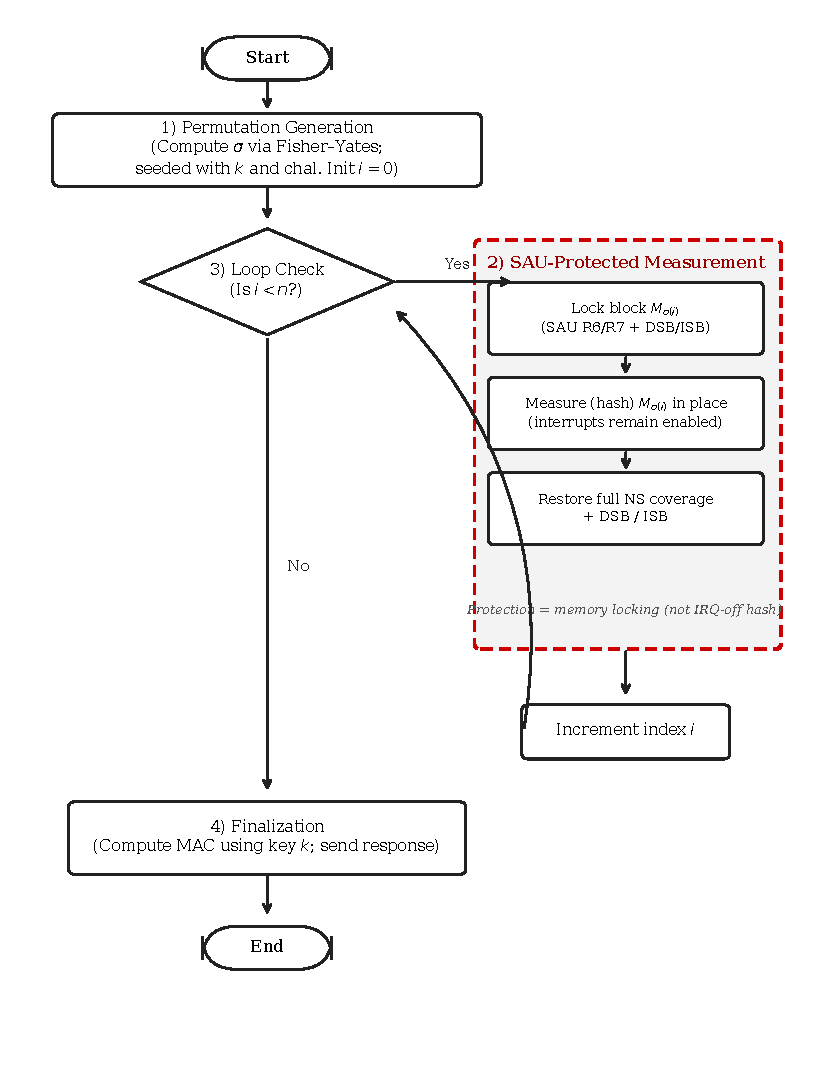
\includegraphics[width=0.92\linewidth]{sau_workflow.pdf}
  \caption{Memory-locking flowchart for \smarmlock{}.
    Each block: lock attribution (brief IRQ off while SAU is updated)
    $\rightarrow$ hash in place with interrupts enabled $\rightarrow$
    restore full NS coverage on $|M|$.
    Integrity during hashing comes from SAU attribution, not from an
    IRQ-off copy.}
  \label{fig:sau_workflow}
\end{figure}

\begin{algorithm}[!ht]
\caption{Memory-Locking Secure Service (\smarmlock)}
\label{alg:sau}
\begin{algorithmic}[1]
\Require $n$ blocks, shuffled indices $\sigma$, data window $M$, key $k$
\State \Call{HMAC.Init}{$k$}
\State \Call{SAU.RestoreWindowNS}{$M$} \Comment{rest state: $|M|$ is NS}
\For{$i \gets 0$ to $n-1$}
  \State $\mathit{blk} \gets M[\sigma(i)\cdot B]$
  \State \Call{DisableInterrupts}{}
  \State \Call{SAU.LockBlock}{\textit{blk}, $B$} \Comment{R6/R7; blk Secure-by-default}
  \State \Call{DSB}{}; \Call{ISB}{}
  \State \Call{EnableInterrupts}{}
  \State \Call{HMAC.Update}{\textit{blk}, $B$} \Comment{in place; interrupts on}
  \State \Call{DisableInterrupts}{}
  \State \Call{SAU.RestoreWindowNS}{$M$}
  \State \Call{DSB}{}; \Call{ISB}{}
  \State \Call{EnableInterrupts}{}
\EndFor
\State \textbf{return} \Call{HMAC.Finalize}{}
\end{algorithmic}
\end{algorithm}

DSB/ISB barriers ensure each attribution change is visible before
hashing or restoring the window.
Non-Secure code cannot lawfully access a block while it is
Secure-by-default, whereas unrelated Non-Secure tasks and interrupts can
still run during the HMAC update~\cite{armv8m-arm}.

\textbf{Security sketch.}
Memory locking makes the selected block Secure-by-default during
hashing, so Non-Secure software cannot lawfully read or write it~(S1
capture integrity without an IRQ-off hash).
Key~$k$ and permutation~$\sigma$ remain in Secure RAM~(S2)--(S3).
Section~\ref{sec:security_summary} summarizes both designs.
We keep the discussion at CPU SAU attribution; bus-master/DMA cases and
post-boot SAU locking used in some TF-M
platforms~\cite{tfm-isolation,tfm2024} are left to the extended version.
The data window $|M|$ lies in Non-Secure flash \emph{outside} the
application code and vector region so SAU updates never remap executable
Non-Secure pages.

\subsection{Security Properties Preserved}
\label{sec:security_summary}

Atomic Copy and \smarmlock{} change \emph{how} each block is captured
for hashing; they do not change SMARM's cryptographic protocol or the
placement of secrets. Both designs therefore preserve (S1)--(S3):
\begin{itemize}
  \item \textbf{(S1) Controlled Execution.}
    Attestation still runs only through Secure/NSC entry points.
    Between blocks, interrupts remain enabled as in SMARM.
    Within a block, Atomic Copy keeps interrupts disabled for the
    entire \texttt{Memcpy}, and \smarmlock{} instead makes the
    selected block Secure-by-default for the duration of the in-place
    hash (after a brief IRQ-off SAU lock/unlock sequence).
    In either case, untrusted software cannot splice into a
    half-captured measurement.
  \item \textbf{(S2) Key Secrecy.}
    The HMAC key $k$ never leaves Secure RAM; neither design exposes
    $k$ to Non-Secure code or to the attested data window.
  \item \textbf{(S3) Private Measurement Order.}
    The permutation $\sigma$ is derived and stored in Secure world and
    is never written to Non-Secure memory. Malware therefore still
    cannot learn the remaining visit order.
\end{itemize}
In short, Atomic Copy and \smarmlock{} reduce the real-time cost of
block capture while retaining SMARM's controlled execution and the
secrecy of $k$ and $\sigma$.

% ================================================================
\section{Evaluation}
\label{sec:eval}

\subsection{Setup}

All measurements use an STM32 Nucleo-144 board with an
STM32L552ZE (Cortex-M33) at $110$~MHz running FreeRTOS.
Block sizes are $B\in\{64,128,256,512,1024,2048,4096\}$~bytes.
For Atomic Copy and baseline SMARM, attested memory size is $512$~KB.
For \smarmlock{} we reserve a $128$~KiB Non-Secure flash data
window $|M|$ at $0\mathrm{x}08060000$--$0\mathrm{x}0807FFFF$, preceded
by a $64$~KiB guard region at
$0\mathrm{x}08050000$--$0\mathrm{x}0805FFFF$ (not attested), and separate
from a $64$~KiB Non-Secure code region at
$0\mathrm{x}08040000$--$0\mathrm{x}0804FFFF$, so memory locking never
covers application vectors or text;
We report real-time availability as the Frequency Accuracy Ratio
(\FAR),
\[
  \mathrm{FAR}=\frac{f_{\mathrm{observed}}}{f_{\mathrm{baseline}}},
\]
following our SMARM baseline study~\cite{smarmplus2026}.
Here $f_{\mathrm{observed}}$ is the execution frequency of a periodic
real-time task $T_{\mathrm{RT}}$ while attestation is active with the
\emph{actual} per-block implementation (interrupts disabled during each
block capture/hash step).
$f_{\mathrm{baseline}}$ is the frequency of $T_{\mathrm{RT}}$ under the
same attestation workload but with interrupts \emph{left enabled} during
block measurement---attestation still runs, but each block step does not
hold the CPU in a non-preemptible window.
Values near $1.0$ indicate that interrupt-disabled block capture
introduces little frequency-level interference relative to that
interruptible baseline.
We measure \FAR{} under $1000$, $100$, and $10$~Hz workloads for all
seven block sizes ($21$ configurations).
At $1000$~Hz, \FAR{} remained approximately $1.0$ throughout.
At $100$ and $10$~Hz, attestation rounds can span multiple task periods
while the metric's integer expected-run count stays at one, so reported
\FAR{} can occasionally exceed $1.0$ without indicating improved
real-time performance; we therefore interpret all tested configurations
as maintaining \FAR{}~$\approx 1.0$.
We report: (i)~TIM2-based \tdis{} for baseline SMARM and Atomic Copy,
(ii)~DWT cycle counts for \smarmlock{} lock+unlock per block (with
interrupts disabled and \texttt{DSB}/\texttt{ISB} around each transition),
and (iii)~\FAR{} under the workloads above. We omit end-to-end runtime
because the \smarmlock{} prototype uses a smaller, separately reserved
$|M|$; such a comparison would conflate algorithmic overhead with measured
size.

\subsection{Non-Interruptibility Cost}

Table~\ref{tab:tdisabled} recalls Atomic Copy versus baseline SMARM.
Atomic Copy reduces \tdis by about $15$--$16\times$ for
$B\geq 128$~bytes.
\smarmlock{} keeps the hash interruptible: the block stays
protected by Secure attribution while HMAC runs, and only the SAU
lock/unlock steps use brief interrupt disable.
Memory locking does \emph{not} eliminate interrupt disablement: each
lock and unlock runs atomically with interrupts off, \texttt{DSB}, SAU
programming, \texttt{DSB}/\texttt{ISB}, then interrupts re-enabled
(Section~\ref{sec:sau}). Table~\ref{tab:tdis_lock} reports DWT cycles
for both transitions combined on our TrustZone-M prototype (mean over
$10$ rounds per configuration). Cycles grow modestly with~$B$
($87$--$143$) because the SAU coverage hole spans more address space,
but remain $\ll 0.01$~ms at $110$~MHz---orders of magnitude below
per-block hashing in Table~\ref{tab:tdisabled}.

\begin{table}[!t]
  \centering
  \small
  \caption{\smarmlock{} \tdis{}: DWT cycles per block (lock+unlock,
    TrustZone-M, mean $\pm$ std over $10$ rounds). Interrupts disabled
    around each transition with \texttt{DSB}/\texttt{ISB}.}
  \label{tab:tdis_lock}
  \setlength{\tabcolsep}{4pt}
  \begin{tabular}{rrr}
    \toprule
    \textbf{$B$ (bytes)} & \textbf{Mean cycles} & \textbf{Std} \\
    \midrule
    64   & 87.0 & 0.0 \\
    128  & 88.0 & 0.0 \\
    256  & 90.0 & 0.0 \\
    512  & 93.9 & 0.3 \\
    1024 & 100.9 & 0.3 \\
    2048 & 114.7 & 0.5 \\
    4096 & 142.9 & 0.7 \\
    \bottomrule
  \end{tabular}
\end{table}

\begin{table}[!t]
  \centering
  \small
  \caption{$t_{\mathrm{disabled}}$: SMARM baseline vs.\ Atomic Copy
    (TIM2, FreeRTOS). Std.\ $<0.003$~ms.}
  \label{tab:tdisabled}
  \setlength{\tabcolsep}{3.5pt}
  \begin{tabular}{rrrrr}
    \toprule
    & \multicolumn{2}{c}{\textbf{Baseline}}
    & \multicolumn{2}{c}{\textbf{Atomic Copy}} \\
    \cmidrule(lr){2-3}\cmidrule(lr){4-5}
    \textbf{$B$} & Mean (ms) & Std & Mean (ms) & Std \\
    \midrule
    64   & 0.062 & 0.001 & $<$0.007$^\dagger$ & --- \\
    128  & 0.120 & 0.001 & 0.007 & --- \\
    256  & 0.237 & 0.001 & 0.015 & --- \\
    512  & 0.472 & 0.002 & 0.029 & --- \\
    1024 & 0.939 & 0.001 & 0.058 & --- \\
    2048 & 1.877 & 0.003 & 0.116 & --- \\
    4096 & 3.749 & 0.002 & 0.240 & --- \\
    \bottomrule
  \end{tabular}

  \smallskip
  \raggedright\footnotesize
  $^\dagger$Completes within one TIM2 tick ($7.27\,\mu$s).
\end{table}

\subsection{Real-Time Availability}

Figure~\ref{fig:far_three} summarizes FAR at $1000$~Hz. Baseline SMARM
degrades for large $B$, whereas Atomic Copy and \smarmlock{}
remain at $\mathrm{FAR}\approx 1.0$ through
$B{=}4096$~bytes.
We additionally swept \smarmlock{} across all seven block sizes at
$10$, $100$, and $1000$~Hz ($21$ configurations); we observed no
$\mathrm{FAR}<1$ (no missed deadlines).
At $1000$~Hz, $\mathrm{FAR}=1.000$ in steady-state rounds; at lower
rates, integer counting occasionally reports $\mathrm{FAR}>1$ when
attestation spans multiple task periods (Section~\ref{sec:eval}).

\begin{figure}[!t]
  \centering
  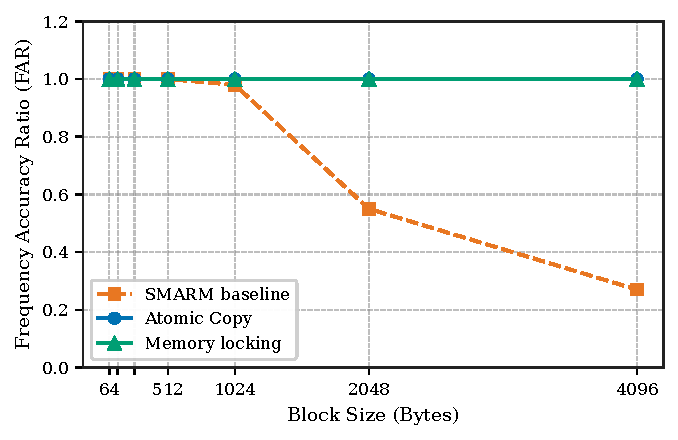
\includegraphics[width=\linewidth]{far_three_1000hz.pdf}
  \caption{FAR under a $1000$~Hz workload. Baseline SMARM loses
    activations for large blocks, whereas Atomic Copy and \smarmlock{}
    maintain FAR~$\approx 1.0$.}
  \label{fig:far_three}
\end{figure}

\subsection{Storage Overhead}

Atomic Copy needs one Secure buffer of size $B$ (up to $4$~KB at
$B{=}4096$).
\smarmlock{} needs no extra measurement buffer.
Both keep
$k$ and $\sigma$ in Secure RAM as in baseline SMARM.
Table~\ref{tab:storage} summarizes the trade-off: Atomic Copy pays a
small, predictable Secure RAM cost; \smarmlock{} avoids that buffer
but requires a dedicated Non-Secure data window $|M|$ that is disjoint
from application code so SAU updates never cover executable pages.

\begin{table}[!t]
  \centering
  \small
  \caption{Storage and layout overhead of the two enhancements.}
  \label{tab:storage}
  \setlength{\tabcolsep}{3.5pt}
  \begin{tabular}{lcc}
    \toprule
    \textbf{Item} & \textbf{Atomic Copy} & \textbf{\smarmlock} \\
    \midrule
    Secure copy buffer & $+B$ (up to $4$~KB) & none \\
    Extra Secure secrets & $k$, $\sigma$ & $k$, $\sigma$ \\
    Dedicated attested window & not required & $128$~KiB (NS flash) \\
    Dynamic SAU regions & none & regions~6/7 \\
    \bottomrule
  \end{tabular}
\end{table}

\subsection{Summary and Design Guidance}
\label{sec:guidance}

Table~\ref{tab:metric_summary} compresses the evaluation into three axes.
Baseline SMARM fails FAR for large $B$ because hashing remains
interrupt-disabled. Both enhancements restore FAR~$\approx 1.0$, but they
pay different costs: Atomic Copy shortens the IRQ-off window to a copy
and consumes Secure RAM of size $B$; \smarmlock{} avoids that
buffer and does not disable interrupts for the hash, but uses brief
IRQ-off SAU lock/unlock steps and a reserved Non-Secure data window
$|M|$.

\begin{table}[!t]
  \centering
  \small
  \caption{Summary of the three SMARM variants on FreeRTOS/TrustZone-M.}
  \label{tab:metric_summary}
  \setlength{\tabcolsep}{2.8pt}
  \renewcommand{\arraystretch}{1.15}
  \begin{tabular}{lp{0.22\linewidth}p{0.22\linewidth}p{0.28\linewidth}}
    \toprule
    & \textbf{FAR} & \textbf{IRQ-off window} & \textbf{Secure RAM / layout} \\
    \midrule
    SMARM baseline &
      Poor for large $B$ &
      Long (per-block hash) &
      No $+B$ buffer \\
    Atomic Copy &
      $\approx 1.0$ &
      Short (per-block copy) &
      $+B$ Secure buffer \\
    \smarmlock &
      $\approx 1.0$ &
      Brief SAU lock/unlock &
      No $+B$; $128$~KiB NS $|M|$ \\
    \bottomrule
  \end{tabular}
\end{table}

\textbf{When to prefer each enhancement.}
Platform guidance typically configures SAU once at boot as part of the
static Secure/Non-Secure map~\cite{armv8m-arm,an5347,cmsis-tz,tfm-isolation},
and production TF-M-style images often lock SAU/GTZC after that
setup~\cite{um2851,tfm2024}.
Our per-block memory locking is not a replacement for that static
partition: it is a short, Secure-only SAU reprogramming of $|M|$ during
attestation.
Choose as follows:

\begin{itemize}
  \item \textbf{Atomic Copy} when Secure RAM of size $B$ is available,
    when SAU must remain locked after boot, when free SAU regions are
    scarce, or when the attested image cannot be isolated from Non-Secure
    code/vectors.
  \item \textbf{\smarmlock} when Secure RAM is tight, a dedicated
    Non-Secure data window $|M|$ can be reserved, and Secure software is
    allowed to reprogram SAU briefly. Because SAU/IDAU govern CPU
    attribution only, DMA or other bus masters still need platform
    controls such as GTZC~\cite{an5347}.
\end{itemize}
The conference prototype leaves SAU unlocked so memory locking can
run; locking policy and DMA-aware enforcement are left to the
extended version.

% ================================================================
\section{Related Work}
\label{sec:related}

\textbf{Classical and shuffled RA.}
SMART~\cite{eldefrawy2012smart}, VRASED~\cite{nunes2019vrased}, and
HYDRA~\cite{eldefrawy2017hydra} use long atomic measurements.
SMARM~\cite{carpent2018smarm}, PRoM~\cite{aman2021prom}, and
HAtt~\cite{aman2018hatt} use shuffled measurement to resist roving
malware while allowing interrupts between blocks. SMARM's original
prototype targeted a seL4/HYDRA stack rather than commodity RTOSes.
A companion report~\cite{smarmplus2026} describes a FreeRTOS/TrustZone-M
instantiation that we use as the experimental baseline; here we evaluate
two per-block capture mechanisms on that stack.

\textbf{Interruptible attestation.}
ISC-FLAT~\cite{isc-flat}, ASAP~\cite{asap}, and IDA~\cite{ida2024}
handle interrupts in control-flow or hybrid attestation. They are
complementary; we target memory-content RA under FreeRTOS.

\textbf{RTOS timekeeping under Secure services.}
Joia Neto \emph{et al.}~\cite{joianeto2026timekeeping} characterize
SysTick loss when Non-Secure RTOS timekeeping is blocked during atomic
Secure-world services on TrustZone-M and propose Secure-world tick
reconstruction. That work is orthogonal to ours: we shorten the
per-block interrupt-disabled window during shuffled measurement rather
than compensating the RTOS clock after long Secure calls.

\textbf{TrustZone-M and SAU.}
TrustZone-M and SAU define CPU security
attribution~\cite{trustzone2025,armv8m-arm,an5347,cmsis-tz}. TF-M and
vendor TFM examples usually set a static SAU map early and may lock it
until reset~\cite{tfm2024,tfm-isolation,um2851}.
We instead apply brief dynamic SAU memory locking during SMARM
measurement as an alternative to copying a block into Secure RAM, and
discuss when that choice is appropriate in Section~\ref{sec:guidance}.

\textbf{Custom hardware.}
LO-FAT~\cite{lo-fat}, LiteHAX~\cite{litehax}, and ATRIUM~\cite{atrium}
remove non-interruptible windows with dedicated hardware. We stay on
unmodified TrustZone-M MCUs.

% ================================================================
\section{Conclusion}
\label{sec:conclusion}

SMARM improves RA interactivity, but interrupt-disabled hashing still
hurts FAR for large blocks on FreeRTOS/TrustZone-M. Atomic Copy cuts
that window to a memory copy and restores FAR~$\approx 1.0$ with a
buffer of size $B$.
\smarmlock{} achieves similar FAR without a copy buffer and keeps
FAR~$\approx 1.0$ across all tested block sizes and $10$--$1000$~Hz
workloads.
Both enhancements preserve SMARM's
security properties~(S1)--(S3): controlled Secure/NSC entry with
integrity of each block capture, secrecy of $k$, and privacy of the
measurement order~$\sigma$. In practice, prefer Atomic Copy when
Secure RAM is available or SAU must stay locked, and prefer \smarmlock{}
when a dedicated data window $|M|$ can absorb brief SAU attribution
changes without an extra Secure buffer.

\bibliographystyle{IEEEtran}
\bibliography{citation}

\end{document}
